% !TEX engine = uplatex
% !TEX producer = dvipdfmx
% !TEX outputDirectory = build
% !TEX moveResultToSourceDirectory = false
\documentclass[10ptj,a4j,fleqn,dvipdfmx,uplatex]{jsarticle}
\usepackage{mine}
\graphicspath{{images/}}

\title{修士論文}
\subtitle{ネオハイパーグレート線形回帰ツヴァイに\\もとづくミリシタにおける最適ユニットの\\選択戦略に関する研究}
\teacher{北沢 志保 教 授\\矢吹 可奈 准教授}
\author{37-123456 イショティハドゥス}
\gakka{ミリシタ学専攻}
\date{平成31年1月31日}

\begin{document}
\maketitle

\null\vfill
\begin{center}
本論文は東京大学大学院アイドルマスター学系研究科に修士号授与の要件として提出した修士論文である.
\end{center}
\vfill
\clearpage

\pagestyle{plain}
\pagenumbering{roman}
\setcounter{page}{1}
% !TEX root = ../main.tex
\section*{内容梗概}

本研究では,アイドルマスターミリオンライブ! シアターデイズにおけるスコアアタック(以後スコアタ)における最適なユニット選択について議論する.
スコアタにおいては,あらゆるユニットに対してモンテカルロ法を適用する手法がとられていた\cite{mirishita-tool}.
本研究では新たに,ユニットのアピール値と特技の組み合わせに対するスコアの回帰方法を提案し,これにネオハイパーグレート線形回帰ツヴァイと名付けた.
実験により,フェス限の伊織・志保・可奈・やよいを持っていればだいたい強いことがわかった.
だから全人類は今度のフェスでフェス限かなしほを引くべきである.


\tableofcontents

% 図目次・表目次は,数が少ないとページ数稼ぎに見えるので,必要ないなら削除したほうがいい
\listoffigures
\listoftables

\clearpage
\pagenumbering{arabic}
\setcounter{page}{1}

% !TEX root = ../main.tex
\section{序論}

\subsection{本研究の背景}
さっさとハイスコアをバリバリ更新したい.

\subsection{本研究の目的}
全部のユニットを試すのは大変なので,アピール値と特技からスコア分布を推定したい.

\subsection{本論文の構成}
こういうのは最後に書け.

% !TEX root = ../main.tex
\section{このフォーマットの使い方}

\subsection{動作環境}

\TeX{}Live 2018の\upLaTeX{}を使っている.
こういうのはなるべく新しいものを使ったほうがいいぞ.

\subsection{ファイル分割}

さすがに大きいと面倒くさそうなのでファイルを分割している.
上手に使いたまえ.

\subsection{フォント}

日本語フォントは各自設定すること.

欧文フォントも日本語に合わせて適当に変えてくれ.
\LaTeX Font Catalogue\footnote{\url{http://www.tug.dk/FontCatalogue/}}などを参考にするとよい.

なおデフォルトはリュウミン+新ゴの組み合わせで綺麗に見えるように作ってある.

\subsection{便利なコマンドなど}

便利なコマンドをちょこちょこ用意したので使ってほしい.

\subsubsection{数式}

argminやargmaxはコマンドを作ってあるのでそれを使うべし.
\begin{verbatim}
    \hat{x} = \argmin_{x} f(x)
\end{verbatim}
\begin{equation}
    \hat{x} = \argmin_{x} f(x)
\end{equation}

括弧は\verb|\paren|,\verb|\sbra|,\verb|\cbra|コマンドを使うと\verb|\left(| / \verb|\right)|などと同じ処理になる.
\begin{verbatim}
    i\hbar\diffp*{\psi\paren{\bm{x},t}}{t}
    = \sbra{\frac{-\hbar^2}{2m}\nabla^2 + V\paren{\bm{x},t}}\psi\paren{\bm{x},t}
\end{verbatim}
\begin{equation}
    i\hbar\diffp*{\psi\paren{\bm{x},t}}{t} = \sbra{\frac{-\hbar^2}{2m}\nabla^2 + V\paren{\bm{x},t}}\psi\paren{\bm{x},t}
\end{equation}

\verb|\abs|とか\verb|\norm|とかもある.
\begin{verbatim}
    \abs{\jacob{x,y}{r,\theta}} = r
\end{verbatim}
\begin{equation}
    \abs{\jacob{x,y}{r,\theta}} = r
\end{equation}

条件付き確率用に\verb|\agivenb|と\verb|\agivenbp|コマンドもある.
pが付いている方は括弧もついでに書いてくれる.
\begin{verbatim}
    p\agivenbp{\bm{x}}{\bm{\alpha}}
    = \frac{\Gamma\paren{\prod^P\alpha_p}}{\prod_p^P\Gamma\paren{\alpha_p}}
      \prod_p^Px_p^{\alpha_p-1}
\end{verbatim}
\begin{equation}
    p\agivenbp{\bm{x}}{\bm{\alpha}} = \frac{\Gamma\paren{\prod^P\alpha_p}}{\prod_p^P\Gamma\paren{\alpha_p}}\prod_p^Px_p^{\alpha_p-1}
\end{equation}

偏微分はdiffcoeffパッケージを使っている.
diffcoeffでググると僕の記事が上の方に出てくるので使うとよい.

\subsection{参照}

\verb|\ref|をするたびに図とか表とか書いてるとキリがないので,ref用のコマンドを作ってある.
\verb|\figref|,\verb|\tblref|,\verb|\eqref|,\verb|\secref|がある.

\verb|\label{fig:hoge}|とすると\verb|\figref{hoge}|とすればいいようになっている.
\figref{kana}はフェス限可奈の特訓前画像.かわいい.フェス限の性能比較は\tblref{fes}に示す.

\begin{figure}
    \centering
    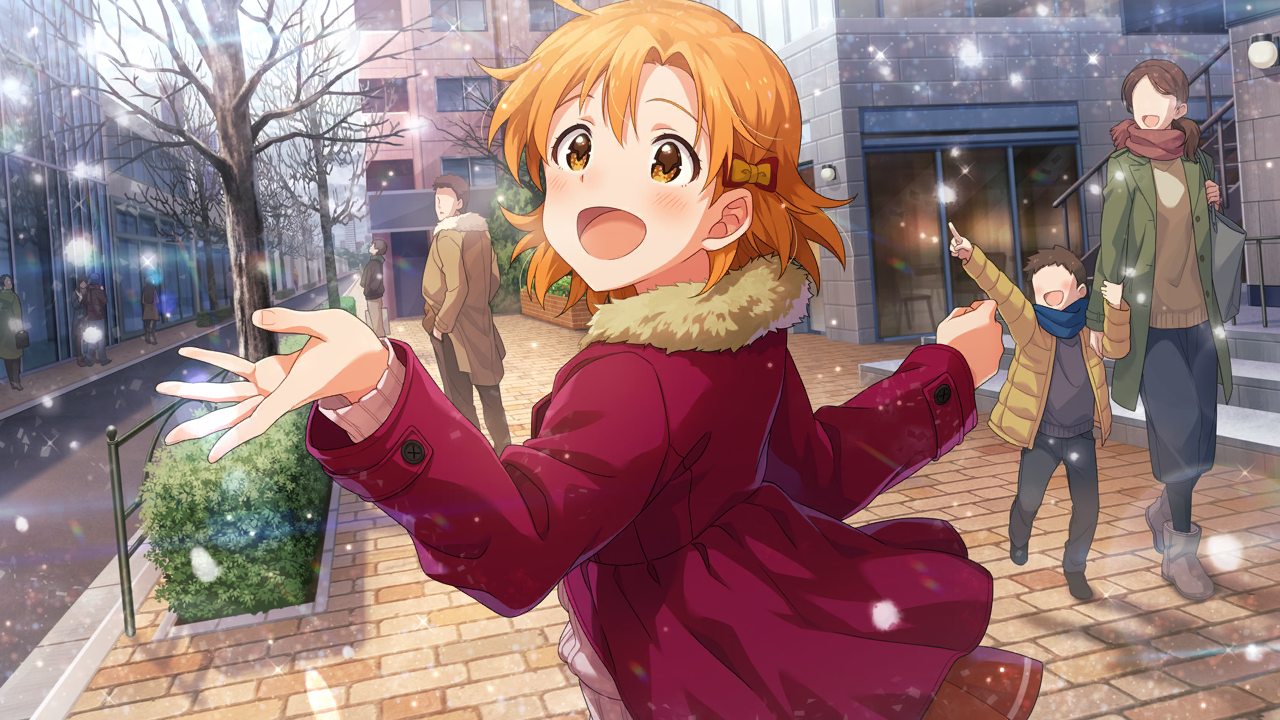
\includegraphics[width=.8\linewidth]{036kan0104_0.png}
    \caption{フェス限矢吹可奈}
    \label{fig:kana}
\end{figure}

\begin{table}
    \centering
    \caption[フェス限やよいおりとかなしほの性能比較]{フェス限やよいおりとかなしほの性能比較(すべて特訓後☆4時).センターに配置すると,特化値が+95\%されることに留意する.こう見ると伊織が弱い.}
    \begin{tabular}{cc|cccc|crcc}
    アイドル & タイプ & Vo & Da  & Vi & 合計 & 特技 & 間隔 & 確率 & 時間 \\ \hline\hline
    矢吹可奈 & Princess & 6433 & 3272 & 9630 & 19335 & コンボナ & 7秒 & 40\% & 4秒 \\
    北沢志保 & Fairy & 3262 & \textbf{9631} & 6454 & \textbf{19347} & コンボナ & 13秒 & 40\% & 7秒 \\
    水瀬伊織 & Fairy & 6452 & 9578 & 3216 & 19246 & コンボナ & 11秒 & 40\% & 6秒 \\
    高槻やよい & Angel & 9601 & 6446 & 3280 & 19327 & コンボナ & 10秒 & 40\% & 5秒
    \end{tabular}
    \label{tbl:fes}
\end{table}

2つ画像を並べるときがときどきあるので,それ用のコマンドも用意してある.
\figref{yayoiori}にその例を示す.

\twofigure{
    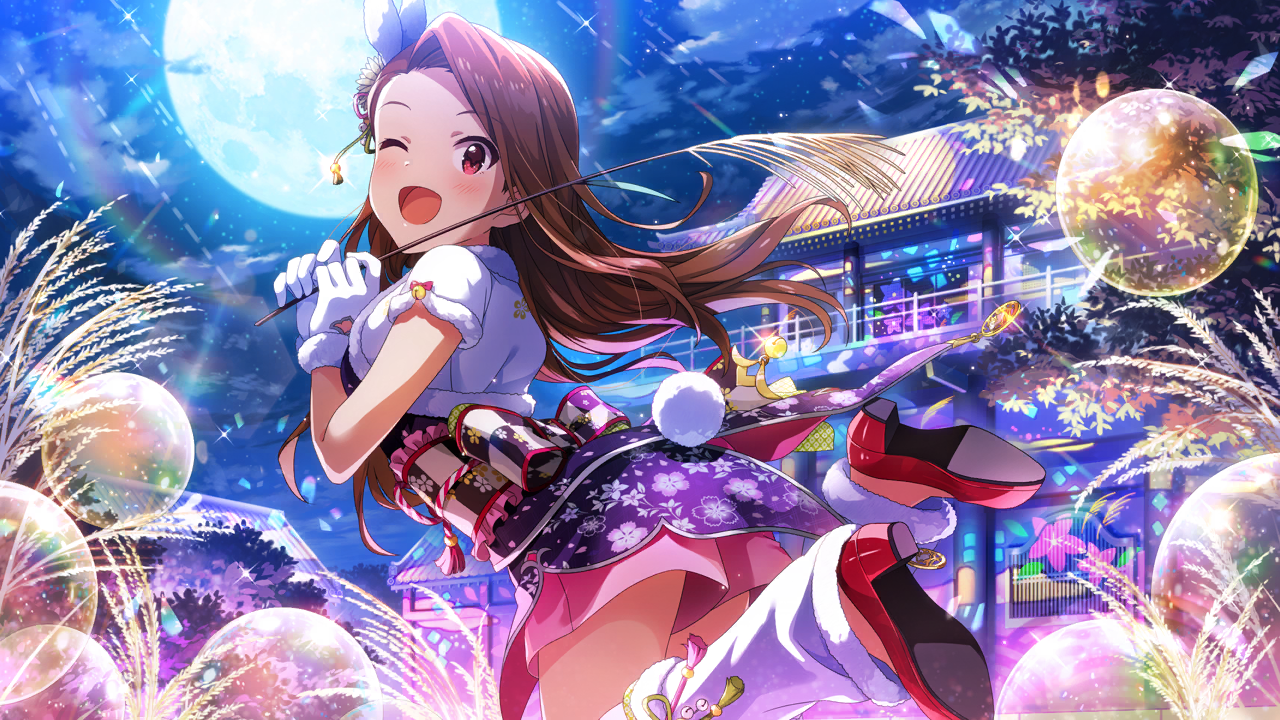
\includegraphics[width=.8\linewidth]{007ior0084_1.png}
    \subcaption{フェス限水瀬伊織}
    \label{fig:iori}
}{
    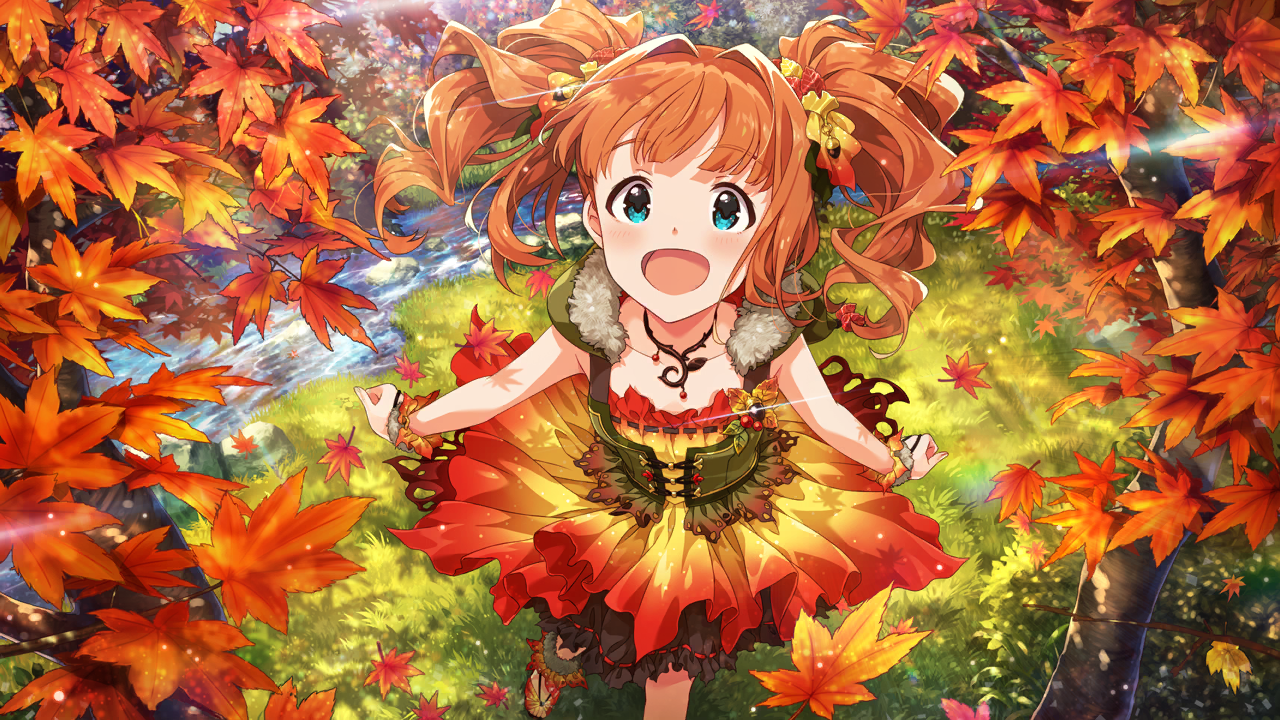
\includegraphics[width=.8\linewidth]{005yay0084_1.png}
    \subcaption{フェス限高槻やよい}
    \label{fig:yayoi}
}{
    \caption[フェス限の伊織とやよいの比較]{フェス限の伊織とやよいの比較(ともに特訓後)}
    \label{fig:yayoiori}
}

\verb|\secref|だけは特殊で,\verb|sec:|を補わないようになっている.
また,章に対するリファレンスは自動的に第$n$章と書かれるので,これだけは普通に\verb|\ref|を使えばよろしい.
すなわち,secrefはsubsection以下のときのみ使う.

\subsubsection{そのほか}

\verb|\enhance{hoge}|で文字列が\enhance{このようにゴシック体になってstrongになる}ようになっている.

\subsection{参考文献について}

参考文献と発表文献を分けて書けるようになっている.
普通にciteすると参考文献に載るようになっており,発表文献のファイルはデフォルトですべて出力されるようになっている.

% !TEX root = ../main.tex
\section{結論}

\subsection{本研究の成果}

みんなかわいいということがわかった.

\subsection{今後の展望}

もっとかわいいカードをいっぱいあつめたい.

% !TEX root = ../main.tex
\section*{謝辞}
ありがとう,箱崎星梨花.私はあなたに出会えてよかった.
あなたともっと色んな世界を見られるように,これからもあなたとずっと歩んでいきたい.

% 謝辞はネタを書く場所でも愛を語る場所でもない.
% この論文を書く上でお世話になった人々への感謝を述べる場所である.
% そのことに留意してひとことひとこと紡いでほしい.
% あと,科研費とか使った人はそういうのも忘れないこと.

\begin{flushright}
    \hspace{0pt}\par
    \thedate\par
    イショティハドゥス
\end{flushright}


\bibliography{references}
\bibliographypubs{publications}

\appendix
% !TEX root = ../main.tex
\section{ネオハイパーグレート線形回帰ツヴァイの導出}
付録は,本文の内容とはちょっと離れているが,論文を構成するのに必要なときに使う.


\end{document}
